\begin{corrige}{devoir1-0004}
  \begin{enumerate}
  \item 
    \begin{enumerate}
    \item  La fonction $f_1$ est une fonction composée. Soit $g(x,y)=x^2+y^2-2$ et $h(\xi)=\ln(\xi)$, alors $f_1=h\circ g (x,y)$. La fonction $g$ est définie partout sur $\eR^2$, et le domaine du logarithme est $\{\xi\in\eR : \xi>0\}$. Le domaine de $f_1$ est alors l'ensemble des points $(x,y)$ tels que $g(x,y)>0$, c'est-à-dire le complémentaire du disque fermé de rayon $\sqrt{2}$ centré dans l'origine. 
 
    \item  La fonction $f_2$ est le rapport entre deux polynômes. Les fonctions polynomiales sont définies partout, mais le rapport est bien défini seulement où le dénominateur est non nul. Le domaine de $f_2$ est donc l'ensemble $\eR^2\setminus {x=y}$. 

    \item  La racine carrée est une fonction définie sur l'ensemble des nombres positifs et en zéro. Ici, comme la racine est au dénominateur, la valeur zéro doit être exclue. Le domaine de définition de $f_3$ est alors donné par la relation $\{(x,y,z) : z^2-x^2-y^2 >0\}$. Il s'agit de l'intérieur d'un cône.   

    \end{enumerate}
  
  \item 

    \begin{enumerate}
    \item   $\displaystyle g_1(x,y)= x+y$, \ref{Figexoquatreuna}, \ref{LabelFigMCQueGF}. ;
    \item   $\displaystyle g_2(x,y)= 1-x^2-y^2$, \ref{Figexoquatreunb}, \ref{LabelFigPHTVjfk}. ;
    \item   $\displaystyle g_3(x,y)= x-y^2$, \ref{Figexoquatreunc}, \ref{LabelFigIWuPxFc}.
    \end{enumerate}
  \end{enumerate}

%TODO : regarder si les figures fonctionnent.


%The result is on figure \ref{LabelFigMCQueGF}. % From file MCQueGF
\newcommand{\CaptionFigMCQueGF}{}
\input{auto/pictures_tex/Fig_MCQueGF.pstricks}

% levelsetsTwo
%The result is on figure \ref{LabelFigPHTVjfk}. % From file PHTVjfk
\newcommand{\CaptionFigPHTVjfk}{}
\input{auto/pictures_tex/Fig_PHTVjfk.pstricks}

% levelsetsThree
%The result is on figure \ref{LabelFigIWuPxFc}. % From file IWuPxFc
\newcommand{\CaptionFigIWuPxFc}{}
\input{auto/pictures_tex/Fig_IWuPxFc.pstricks}

%\newcommand{\CaptionFiglevelsetsOne}{}
%\input{auto/pictures_tex/Fig_levelsetsOne.pstricks}

%\newcommand{\CaptionFiglevelsetsTwo}{}
%\input{auto/pictures_tex/Fig_levelsetsTwo.pstricks}
 
%\newcommand{\CaptionFiglevelsetsThree}{}
%\input{auto/pictures_tex/Fig_levelsetsThree.pstricks}

 \newpage

\begin{figure}
    \subfigure[]{
            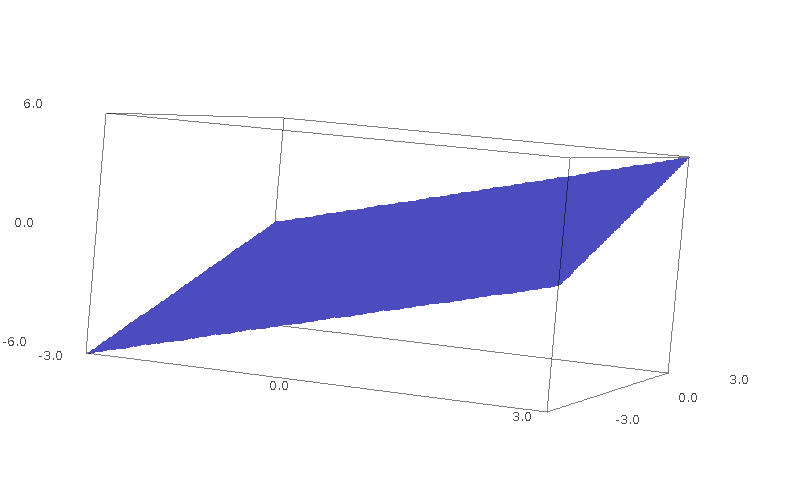
\includegraphics[width=5cm]{pictures_bitmap/exoquatreun.png}
        \label{Figexoquatreuna}
  }
    \subfigure[]{
            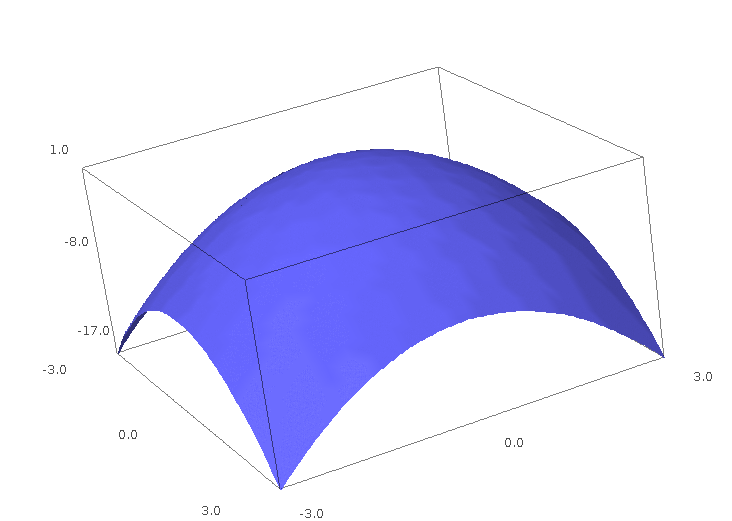
\includegraphics[width=5cm]{pictures_bitmap/exoquatredeux.png}
        \label{Figexoquatreunb}
  }
    \subfigure[]{
            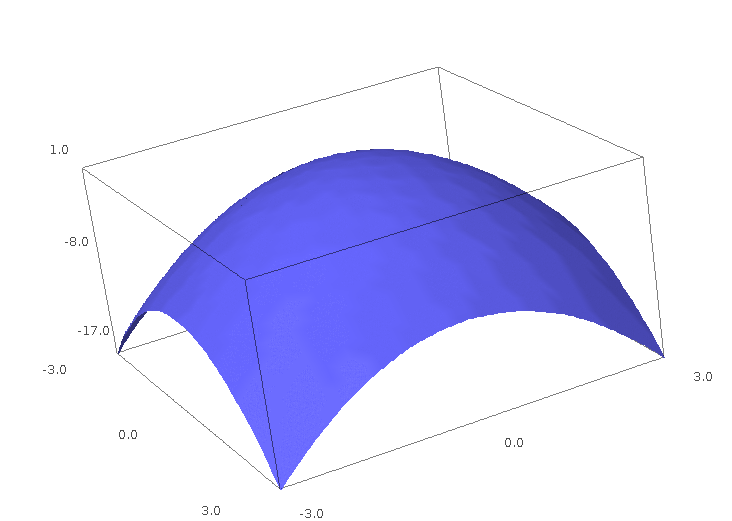
\includegraphics[width=5cm]{pictures_bitmap/exoquatredeux.png}
        \label{Figexoquatreunc}
  }

  \caption{Des dessins pour l'exercice \ref{exodevoir1-0004}}
  \end{figure}


\end{corrige}
